\documentclass{article}
\usepackage{graphicx}
\usepackage{url}
\hyphenation{SiDiff}


\providecommand{\internal}[1]{#1}



\begin{document}

\title{The SiDiff Framework
\\ An Introduction}

\author{
       Pit Pietsch\\
       Software Engineering Group\\
       University of Siegen, Germany\\
       pietsch@informatik.uni-siegen.de
}

\maketitle
\newpage

\tableofcontents
\newpage

\section{Disclaimer}
\label{secdisclaimer}
This paper is an introduction to the model comparison framework SiDiff, which was developed and is maintained by the Software Engineering Group 
of the University of Siegen. Please note that some of the referenced work is only available in german language. \newline 

\section{General Overview}
\label{secintro}

SiDiff is an meta model independent approach to model comparison. It is primarily based on the notion of similarity between model elements, but covers 
other approaches like id-based or signature-based model comparison as well. 
The main advantage of SiDiff is that it offers a highly configurable environment and is therefore easily adaptable to any model type where a given 
occurrence of a model can be represented in a graph-like structure. The intention of this paper is to give the reader an overview of the 
basic concepts behind the SiDiff-Framework. So this text makes no claim of completeness. The reader should be aware that additional 
functionality and optimizations exist within the framework which are not mentioned here. Furthermore the text abstracts any concrete implementation 
concepts and technical details as long as the comprehensibility is not endangered.   \\

The paper is structured as follows: Section \ref{secmodels} is a brief introduction into the importance of models and how models are processed by SiDiff. 
Section \ref{sechistory} gives a brief overview of the history of SiDiff. It is explained 
under what objectives the framework was initially developed and it describes the modifications that have been made over time to evolve the first prototype to the 
meta model independent and highly flexible framework for model comparison SiDiff is today. 
Section \ref{secsidiffcomps} explains the different components and concepts used by SiDiff. This includes, but is 
not limited to, aspects of the typical model comparison process, how SiDiff can be configured and adapted to different domains, 
the algorithm used for difference calculation as well as the representation of the computed difference. \\

The reader may feel free to contact us directly for more information about our work and the SiDiff-Framework. 

\section{Models and Modelmanagement}
\label{secmodels}

The importance of models vastly increased in the last decade. Models grew from mere documentational accessories to essential first level artifacts within the development processes of many 
domains. The most important facilitator in this regards was the rise of the model driven software development paradigm (MDSD) and its companying and closely related 
concepts of model driven engineering (MDE) and model driven architecture (MDA). But the usage of models is nowadays not only limit to technical domains like software engineering, but models are also utilized in 
less formal domains as well. One example are business process models that are used by companies to represent the knowledge over vital and reoccuring processes. 
For the user who has to deal in his daily work with such models it is often interesting, sometimes even crucial, to identify the changes 
that exist between two versions of model. For example when a class diagram was concurrently modified by different users it is vital to recognize if the changes in the two versions conflict or if the models can simply be merged. Model comparison can assist these tasks by identifying the corresponding parts of the models, derive the difference and present the difference to the user in a way that supports him in his work. \\

Model mangement in SiDiff is based on the meta model of the Eclipse Modeling Framework (EMF), called Ecore. Technically Ecore is a meta meta model, because it 
is itself an EMF/Ecore model\footnote{But this is just a scientific distinction and not really important for the comprehensibility of this text}. The advantage in using EMF/Ecore stems from the 
fact that EMF offers built in, easy to use runtime support and persistence mechanisms for models, as well as an an API to generically manipulate instances of models. Furthermore the Eclipse 
Modeling Project established itself in the last couple of years as de-facto standard for the model community and is supported by many vendors. Also additional bridges 
for many domains into the realm of EMF exist.\\ 

In the context of the SiDiff framework, Ecore is used as a meta meta model to describe the different domain models (or meta models) of interest, e.g. the Unified Modeling Language (UML), Matlab/Simulink or the Business Process Model Notation (BPMN). Instances\footnote{The terms instance, concrete model, model and document are used interchangeable during this paper} of these meta model models of these domain models, e.g. two class diagrams, are then compared by the framework, the correspondences and differences are computed and the results are further processed by the user or another software.  


\section{History of SiDiff}
\label{sechistory}

The beginning of SiDiff can be traced back to the year 2003, when an early predecessor of todays SiDiff was 
presented in \textit{Differences between Versions of UML Diagrams} \cite{Ohst03DiffVer}. 
While in \cite{Ohst03DiffVer} several important topics related to model comparison were 
addressed, e.g. how to abstract from irrelevant changes, how to visualize important changes appropriately and how to 
identify and deal with structural changes of the given models, this first approach had a couple of limitations. One for example is 
that the proposed approach is only applicable to UML diagrams. Furthermore it makes use of persistent identifiers to identify the elements 
within the models and is tool-dependent, i.e. the models had to be stored in a H-PCTE database.

To address the shortcomings of the prototype an generic differencing tool \cite{Weh04SiDiff} was developed in 2004. While 
this prototype still had its focus on the comparison of UML class- and activity-diagrams, 
the underlying data model was designed in a way that additional types of UML diagrams and models complying to meta models from different domains 
could be easily supported as well. Based on this groundwork the SiDiff framework was build and introduced by Kelter in 
\textit{A Generic Difference Algorithm for UML Models} \cite{Kel05DiffAlg} in the year 2005.  

In the following years SiDiff was continuously improved. Because of the rise of the model-driven engineering paradigm and 
the resulting increased need for model comparison new domains of application became available. 
As of today there is a working branch of SiDiff that supports comparison of MATLAB/Simulink diagrams \cite{Kel07Mate, Sch08ConsDiff}. MATLAB/Simulink 
is a tool for modeling and simulation of dynamic systems that is used by engineers in fields like signal processing, image 
processing and control design. Another branch is currently adapting SiDiff for the ASCET-Software family, a toolbox 
used in the context of model driven development of embedded software for automotive systems. Furthermore ongoing efforts are made to 
explore new areas of application, e.g. using SiDiff for finding similarities between sentences of a constraint language \cite{Bild09SoftRe} or the 
comparison of molecular graphs \cite{Gra08MolGra} in the field of chemo-informatic.      

Besides the described transfer into new domains another main focus of research is to improve and speed up the comparison of 
very large models. Several approaches in this regard have been investigated and implemented \cite{Tre07DiffComp, Pie08FP}. Other fields of 
interest of our chair include, but are not limited to, research on how models change over time and how to trace model elements through different versions 
of a model \cite{Wen08ModEvu}, as well as visualization aspects of model comparison, e.g. with the help of polymetric views \cite{Wen08ScaVis} or 
3D visualization of software metrics \cite{Koch09, Wenzel09}.

In early 2009 SiDiff was completly overhauled. The SiDiff framework is now implemented based on the OSGi-Platform. This 
allows for easy exchange of the different components in case the given application context warrants it. Furthermore the 
properitary, internal data format used in the old version has been disposed. Representation of the models are now based on EMF/Ecore and SiDiff can compare any 
Ecore based models readily. EMD/Ecore emereged as a defacto-standard in the model community and is already used in many modeling related applications 
and bridges to other modeling domains exist. Therefore SiDiff can now be integrated with a multitude of additional applications and domains.  
 

\section{The SiDiff Components}
\label{secsidiffcomps}

% \sectio{Model Comparison with SiDiff}
% \label{secmodelcomparison}
% SiDiff can best be described as a open framework with a set of libraries related to model differencing. SiDiff is applicable to all graph-based modelling languages for that 
% an Ecore complient representation of the given meta model exists. Different than other comparison approaches SiDiff supports, but does not rely on persistent identifiers, 
% unique names or element signatures for establishing correspondences between elements. At it's core is a highly configurable matching algorithm that can 
% be adapted to any specific application context. 



The general approach of comparing two models is as follows. At first the models are usually available as 
textual or binary documents, often specified within XMI or a proprietarian vendor format. 
In case they do not directly exist as instances of EMF/Ecore based domain models, 
SiDiff reads and transforms the given input documents for further processing. Once the models are 
accessible for the SiDiff kernel they can be compared and the resulting difference 
information is visualized to the user or used as input for further applications. 
Figure \ref{figarchitecturecomps} shows the process of a typical 
model comparison as well as the main components that are involved. The single components 
will be described in more detail in the next paragraphs.

\begin{figure}[h]
\centering
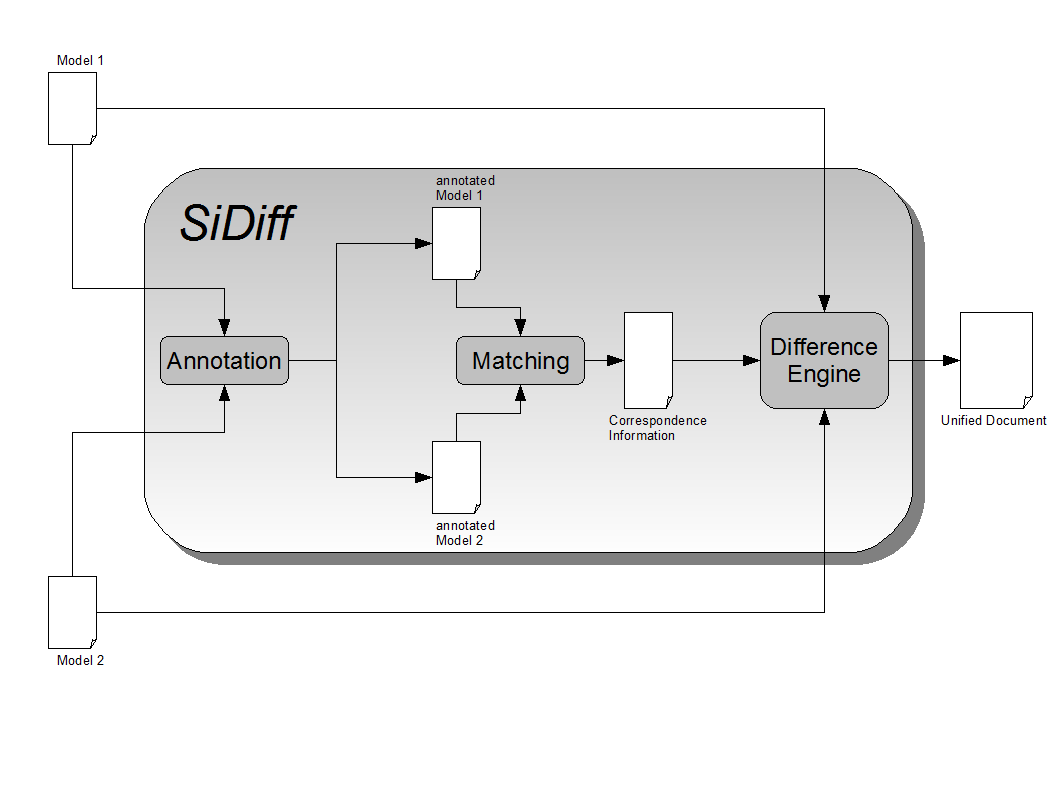
\includegraphics[width=\linewidth]{sidiffworkflow.png}
\caption{Model Comparison Components}
\label{figarchitecturecomps}
\end{figure}

For more detailed information on the different components and the comparison process see \cite{Kel05DiffAlg, Tre07DiffComp, Weh04SiDiff}.

\subsection{Annotations}
\label{secannotations}

Before the actual comparison processes is triggered, the models to be compared can be enriched with additional 
information by the means of annotations. Every element of the model is visited once and one or more annotations are computed and attached 
to the element. Which annotations are computed is defined within a configuration file. This mechanism can be used to calculate 
specific static, derived information about elements that can be used in the comparison workflow, like software metrics, hash-values and 
path-information.


\subsection{Matching}
\label{secmatching}
 
In the second step of the model comparison correspondences between elements are established. 
SiDiff is fully able to support the three major state of the art matching strategies, 
i.e. ID-based, signature-based and similarity-based matching. It is also possible to combine the different approaches where 
applicable, e.g. using a id-based matching first and apply a signature based matching on 
the remaining unmatched model elements. This allows to capitalize on adequate features of a given meta model 
without sacrificing any applicability. The different strategies are now discussed in more detail.    

\subsubsection{ID-Based Matching} 
This matching approach is the most trivial and fastest. Every nodes has by definition a persistent and unique ID and 
nodes that have the same ID are deemed corresponding and therefore are matched. It has to be noted that not every 
domain and tool is designed to support such IDs, This approach also usually fails when tools from different vendors 
are used in the development process of the models.    

\subsubsection{Signature Based Matching}
In some application contexts the single elements do not have a unique ID, but share characteristics 
that can be used as a definite discriminator and thus signature based matching can be applied. The signature of each element is 
usually computed during the annotation phase in form of a hash-value over the relevant characteristics. In case that  
the signature can be used like an unique ID elements that share the same signature are matched at once. If the signature 
is only an necessary implication for a possible matching it can be used used to downsize the search space significantly 
and only promising elements undergo any further similarity analyses.

\subsubsection{Similarity Based Matching}
Besides the already mentiones and rather trivial approaches to model comparison, SiDiff is also capable to establish matches between elements 
based on the notion of similarity. This is an advantage because not every context of application offers the potential to use the previously 
mentioned simplifications to establish correspondes between elements. Within a similarity-based approach, the similarity between two elements is 
usually determined by either local attributes or by elements in the near proximity, e.g. referenced- or child-elements. SiDiff offers a 
wide range of functions for computing similarities values based on such characteristics. New functions can be added easily if an application context 
warrants it.

A similarity function calculates the similarity value between two element properties. It returns the computed similarity as a 
float value between 0 (no similarity) and 1 (equality). Because the similarity between two elements usually depends not only on one, but on 
multiple properties a set of similarity functions can be defined for any given element type. To further reflect the fact that some properties may have a higher 
significance for the computation of the similarity as others, weights must be assigned.

The similarity between two elements is therefore defined as the weighted arithmetic mean of the
similarities of the relevant properties. 
\[ sim_{e_1,e_2} = \sum_{p \in P} w_p \cdot \mathrm{compare_p(e_1, e_2)}, \]
where $e_1$ and $e_2$ are the elements to be compared, $P$ is the set of
similarity-relevant properties, $w_p$ gives the weight of property $p$ and
$compare_p$ is the compare function for property $p$. 

To ensure that only elements that share a certain similarity are matched a 
threshold has to be defined for each element type. Only Elements with a similarity above the treshold are deemed as similar. Thus it prevents that matchings 
between elements that share only a small similarity are established. An example configuration for the (pseudo-)element type \textit{Element} can be 
found in table ~\ref{tabsimconfig}. \\

\begin{table} [h]
\centering
\begin{tabular} {l | c}
\hline
Node Type & \textit{someElement} \\
Threshold & 0.7 \\ \hline \hline

Criterion & Weight \\
\hline
Similar value for attribute \textit{name} & 0.5 \\
Equal value for attribute \textit{state} & 0.1 \\
Similar elements following outgoing \textit{Edge type A} & 0.1 \\
Similar elements following incoming \textit{Edge type B} & 0.1 \\
Matched parent element & 0.2 \\
\end{tabular}
\caption{Example Similarity Configuration}
\label{tabsimconfig}
\end{table}

\subsection{Difference Engine}
\label{secunidoc}
The difference engine takes the two input models and the computed correspondences to create an unified XML-document. This document can be seen as 
the output of the comparison. It consists of all elements of the two original models (corresponding elements are only contained once), as well 
as the difference information that was computed during the comparison process.\\

The difference between two documents can be easily deduced: 
\begin{itemize}
\item structural difference: Elements that have no correspondence in the document, i.e. insertion and deletions
\item attribute difference: Two elements that correspond, but differ in their attribute values
\item reference difference: Two elements that correspond, but differ in their references
\item move difference: Two elements that correspond, but have different parent elements 
\end{itemize}

The differenct categories of difference are also depicted in Figure \ref{figdiff}. While the unified document contains all the information about the calculated difference, the chosen final 
visualizations depends on the given context, the next processing step and the domain and application specific 
needs of the user. 

\begin{figure}[h]
\centering
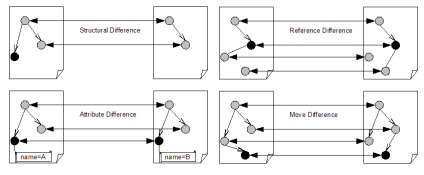
\includegraphics{differences.png}
\caption{Categories of Difference}
\label{figdiff}
\end{figure}

\section{Conclusion}
\label{secconclusion}
In this paper we have outlined the meta model independent comparison framework SiDiff. It is a highly configurable approach to model 
comparison based on the notion of similarity between model elements. 
Its configurability allows the user to define the similarity between elements as simple or as complex 
as needed for any given context. As of today, SiDiff supports a wide range of different model types from various fields of application. 
The current version of the framework is already used by partners in business and science.  
Therefore SiDiff is not only offering a theoretical concept or research implementation, but a proven to work workbench for model 
comparison. We are constantly looking to refine the current SiDiff framework and its capabilities and are looking 
for new fields of application as well.\\  

Feel free to contact us directly if you are interested in more information about our work and the SiDiff model comparison framework. 

\bibliographystyle{abbrv}
\bibliography{primary}

\end{document}